\documentclass{article}

\usepackage{graphicx}
\usepackage{caption}
\usepackage[x11names]{xcolor}
\usepackage[nameinlink]{cleveref}

\setlength{\textwidth}{6.5in} % Increase the line width
\setlength{\oddsidemargin}{0in}
\setlength{\evensidemargin}{0in}
\setlength{\topmargin}{0in}
\setlength{\headheight}{0in}
\setlength{\headsep}{0in}
\setlength{\textheight}{9in}

\title{Supplementary Materials - EnsembleDashVis Views and Volunteers: A Retrospective and Early History}

\author{Qiru Wang\thanks{e-mail: qiru.wang1@nottingham.ac.uk}\\ %
\scriptsize Visualization and Graphics Group \\
        \scriptsize University of Nottingham %
\and Robert S. Laramee\thanks{e-mail: robert.laramee@nottingham.ac.uk}\\ %
\scriptsize Visualization and Graphics Group \\
        \scriptsize University of Nottingham 
}

\date{}
\begin{document}
\maketitle

\section{High-Resolution Figures}

High-resolution figures for all five visual designs described in Section 4 of our paper are included here.

\begin{figure}[h!]
    \centering
    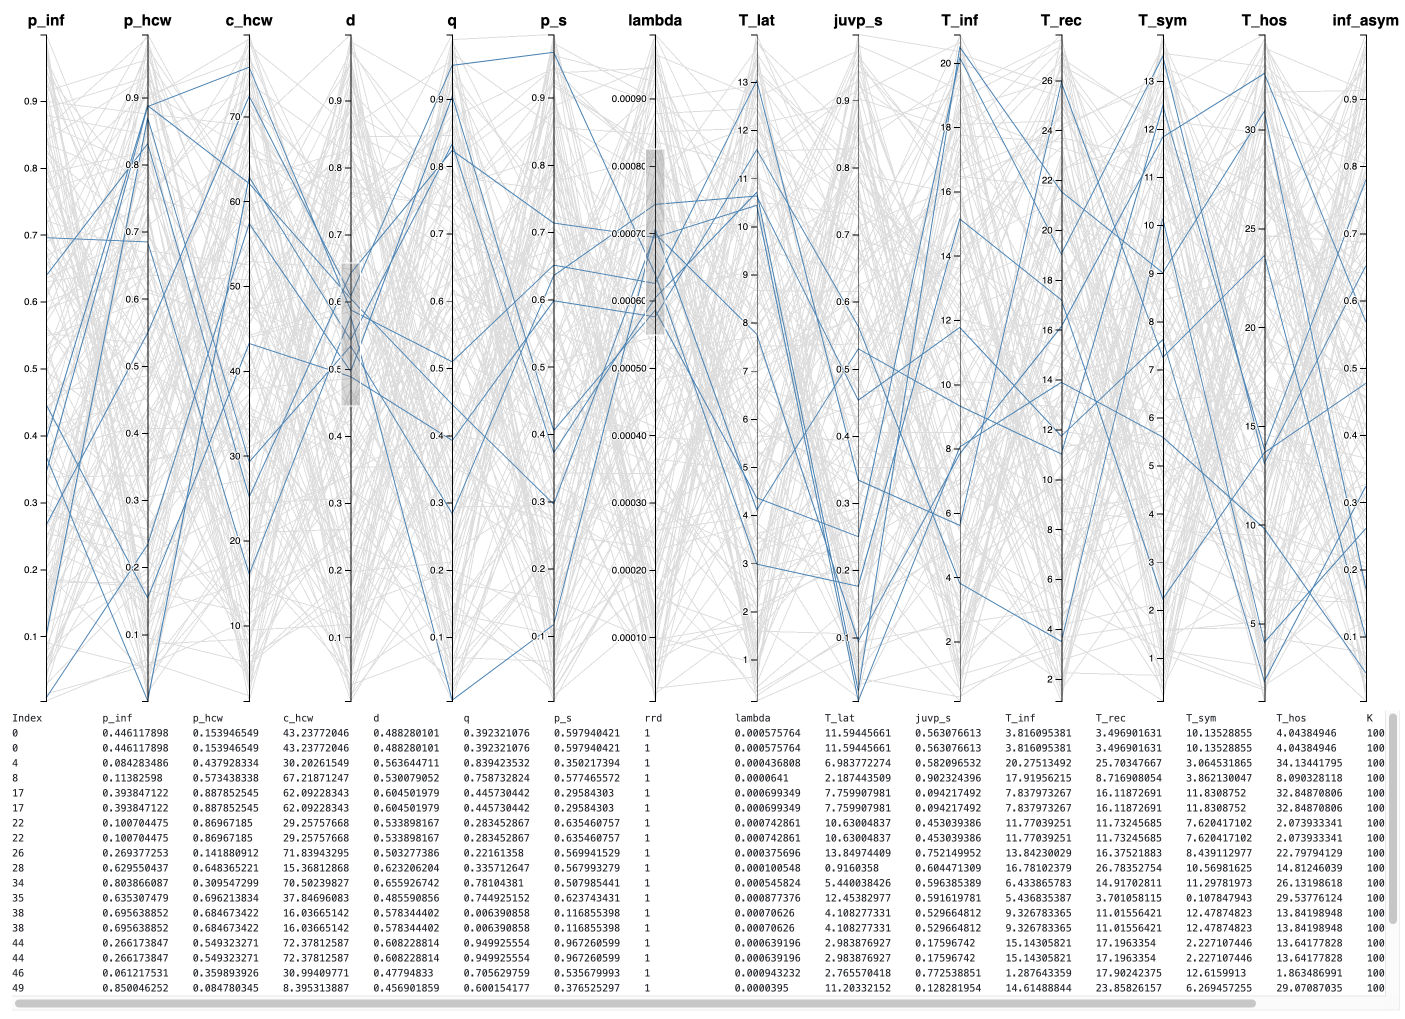
\includegraphics[width=\linewidth]{figures/pc1.png}
    \caption{The first visual design, a parallel coordinates plot depicting all 160 input configurations of the model, was completed on 5 Nov 2020. 
    Each axis represents an input parameter, the y-axis represents the value of the parameter, and each polyline represents one input configuration.
    The table below shows the configuration details.
    }
    \label{fig:pc1}

\end{figure}


\begin{figure}[h!]
    \centering
    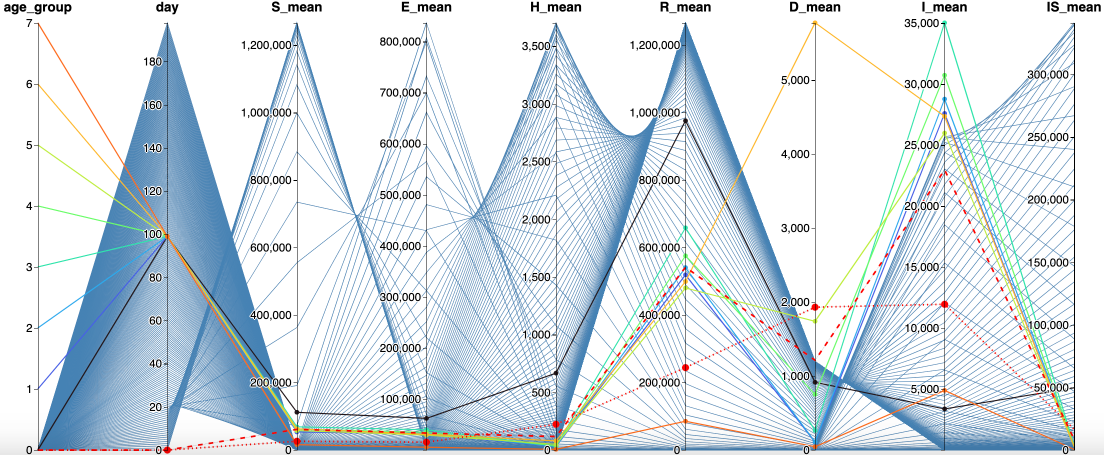
\includegraphics[angle=90,height=0.9\textheight]{figures/pc2.png}
    \caption{A parallel coordinates plot depicting the model outcomes by age group. As requested by the modelers, the mean value of 160 predictions generated by each input configuration, as well as for each age group, was computed and rendered here. Each axis represents one variable from the outcome and \textcolor{SteelBlue4}{its value}.
    Each age group is mapped to a color, the dashed red line {\textcolor{red}{\rule[0.3ex]{0.2cm}{0.5pt}\hspace{0.1cm}
    \rule[0.3ex]{0.2cm}{0.5pt}\hspace{0.1cm}
    \rule[0.3ex]{0.2cm}{0.5pt}\hspace{0.1cm}}}
    represents the average value, and the dotted red line \textcolor{red}{\textcolor{red}{
    \rule[0.3ex]{0.05cm}{0.1pt}\hspace{0.05cm}
    \rule[0.3ex]{0.05cm}{0.1pt}\hspace{0.05cm}
    \rule[0.3ex]{0.05cm}{0.1pt}\hspace{0.05cm}}} represents the standard deviation.}

\end{figure}




\begin{figure}[h!]
    \centering
    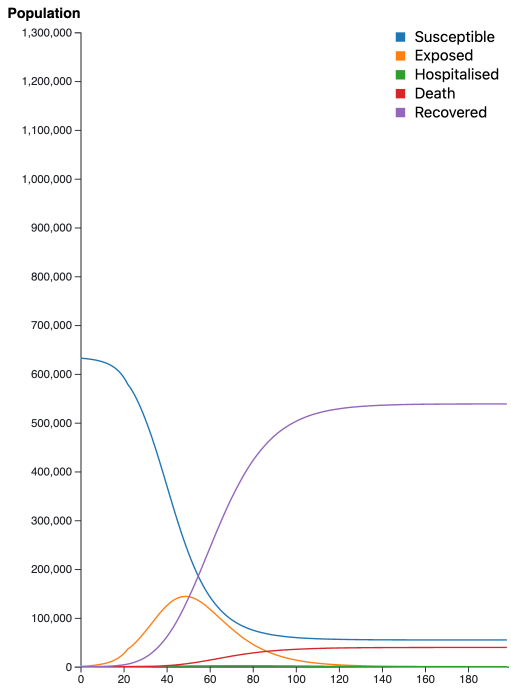
\includegraphics[width=\linewidth]{figures/1st-line.png}
    \caption{A line chart depicting the model outcomes.
    The x-axis of the chart corresponds to the number of days since the first date in the Scottish dataset, while the y-axis represents the population.
    To differentiate between different population categories, a color map was incorporated: \textcolor{DodgerBlue1}{susceptible}, \textcolor{Chocolate1}{exposed}, \textcolor{Green4}{hospitalized}, \textcolor{red}{recovered}, \textcolor{DarkOrchid1}{death}, \textcolor{LightSalmon4}{asymptomatic}, and \textcolor{HotPink1}{symptomatic}.
    The focus+context technique is used here to highlight the outcome of the current configuration, while the grey lines represent other outcomes. On day 20, there is an unusual spike which was later identified as caused by an error in the model.
    }
    \label{fig:1st-line}

\end{figure}


\begin{figure}[h!]
    \centering
    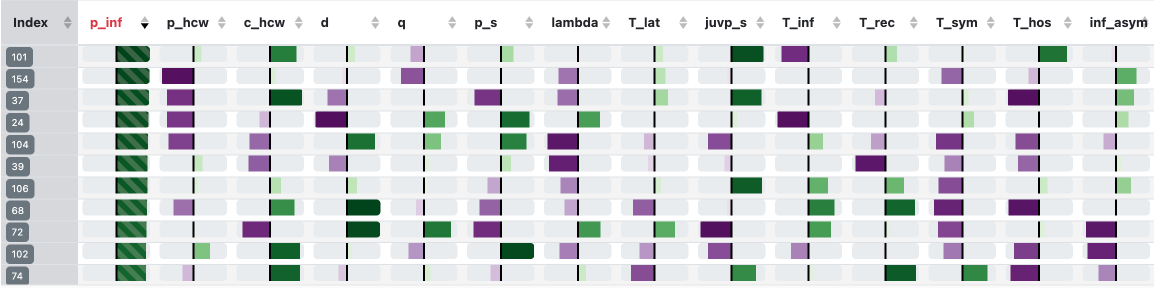
\includegraphics[angle=90,height=0.9\textheight]{figures/table.png}
    \caption{The table view depicting all 160 input parameter configurations.
    The view enables the modelers to sort parameter values and identify interesting configurations.
    Each row represents an input configuration, and each column represents an input parameter.
    Upon clicking on a row, the line chart in \Cref{fig:1st-line} is updated to display the corresponding model outcomes.
    Clicking on the column header sorts the table by the parameter values.
    }
    \label{fig:table-view}

\end{figure}

\begin{figure}[h!]
    \centering
    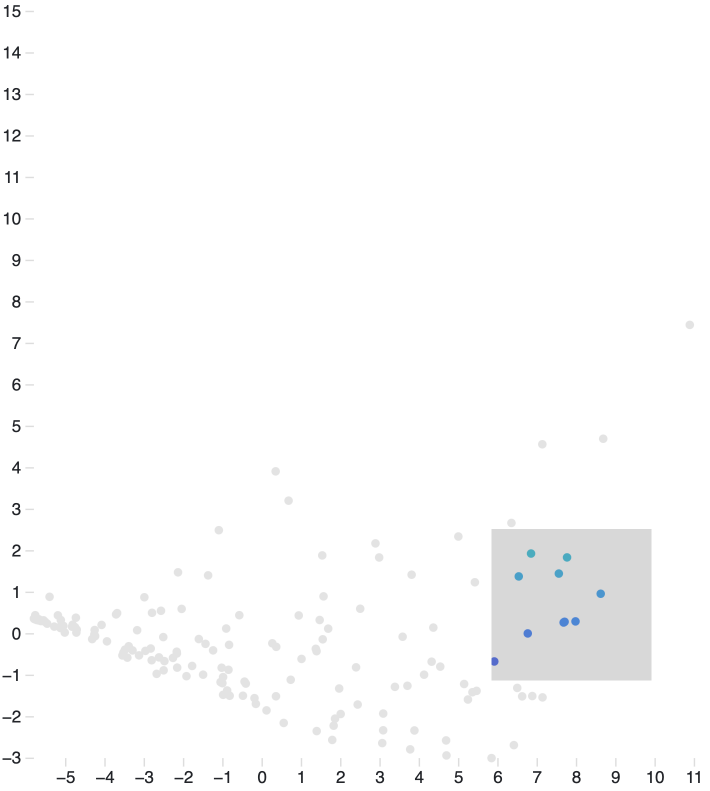
\includegraphics[width=\linewidth]{figures/pca.png}
    \caption{A scatterplot depicting the PCA outcome from another VIS volunteer group, was added upon request by the modelers. Upon brushing, the selected configurations are highlighted in the table view in \Cref{fig:table-view}.
    }
    \label{fig:pca}

\end{figure}

\end{document}